\newpage
%\appendix
\section{Proofs of Theorems~\ref{lemma:warmnum1} and \ref{lemma:warmnum2}}
\label{appendixa}
In this section, we describe the proof details of Theorem~\ref{lemma:warmnum1} and Theorem~\ref{lemma:warmnum2}.

For the following calculation,
 all the probabilities are in $[0,1]$.
 %$0 \leq P_{a|S_{c}} \leq 1$, $0 \leq P_{S_{\bar{c}, a}|S_{\bar{c},\bar{a}}} \leq 1$, $0 \leq P_{S_{\bar{c}, a}|S_{\bar{c},\bar{a}}}^{\ominus} \leq 1$, $0 \leq P_{S_{\bar{c}, a}|S_{\bar{c},\bar{a}}}^{\oplus} \leq 1$, $0 \leq P_{w}^{\ominus} \leq 1$, $0 \leq P_{w}^{\oplus} \leq 1$
 %and $0 \leq P_{e|S_{c}} \leq 1$.

\subsection{Proof of Theorem~\ref{lemma:warmnum1}}
\label{appendixa1}
To prove the Theorem~\ref{lemma:warmnum1}, we need to compare $E(T^{\ominus})$ with $E(T)$.
So we get the Formula~\ref{equ:tpc1}, and estimate if it is greater than $0$.
By combing Equation~\ref{equ:pic} and ~\ref{equ:pil}, we get Equation~\ref{equ:ypwarm1} and \ref{equ:detail1}.

%\begin{footnotesize}
\begin{equation}
\label{equ:ypwarm1}
\begin{split}
%\footnotesize
%\scriptsize
y(&P_{w}^{\ominus}) = -P_{S_{\bar{c}, a}|S_{\bar{c},\bar{a}}}P_{S_{\bar{c}, a}|S_{\bar{c},\bar{a}}}^{\ominus} \\
&-P_{e|S_{c}}(P_{S_{\bar{c}, a}|S_{\bar{c},\bar{a}}}^{\ominus}+P_{a|S_{c}}-P_{a}^{\mathfrak{3}\mathcal{L}}))*P_{w}^{\ominus} \\
& +  P_{e|S_{c}}P_{S_{\bar{c}, a}|S_{\bar{c},\bar{a}}}^{\ominus}(1-P_{a|S_{c}})+P_{S_{\bar{c}, a}|S_{\bar{c},\bar{a}}}^{\ominus}P_{S_{\bar{c}, a}|S_{\bar{c},\bar{a}}}\\
& - P_{e|S_{c}}P_{S_{\bar{c}, a}|S_{\bar{c},\bar{a}}}(1+P_{S_{\bar{c}, a}|S_{\bar{c},\bar{a}}}^{\ominus}-P_{a}^{\mathfrak{3}\mathcal{L}}) \,
\end{split}\end{equation}

\begin{equation}
\label{equ:detail1}
\begin{split}
E(T^{\ominus}) - E(T) = &\frac{y(P_{w}^{\ominus})P_{e|S_{c}}T_{d}}{A_{L}*B_{L}}
\end{split}\end{equation}
%\end{footnotesize}
where
\begin{equation*}
\begin{split}
&A_{L}=P_{e|S_{c}}(1+P_{S_{\bar{c}, a}|S_{\bar{c},\bar{a}}}^{\ominus}-P_{S_{\bar{c}, a}|S_{\bar{c},a},\bar{w}}^{\ominus})\\
&\ \ +(1-P_{e|S_{c}})P_{S_{\bar{c}, a}|S_{\bar{c},\bar{a}}}^{\ominus}P_{w}^{\ominus}+(P_{S_{\bar{c}, a}|S_{\bar{c},a},\bar{w}}^{\ominus}-P_{a|S_{c}})P_{e|S_{c}}P_{w}^{\ominus} \\
&B_{L}=P_{S_{\bar{c}, a}|S_{\bar{c},\bar{a}}}+P_{e|S_{c}}(1-P_{a|S_{c}})
\end{split}\end{equation*}
In the Markov state transition diagram,
\begin{equation*}
\begin{split}
&P_{S_{\bar{c}, a}|S_{\bar{c},a}^{\bar{w}}}^{\ominus}=P_{e|S_{\bar{c}, a}}^{\ominus}P_{a|S_{\bar{c}, a}}^{\ominus}+(1-P_{e|S_{\bar{c}, a}}^{\ominus})P_{a|S_{c}} .
\end{split}\end{equation*}
It can be seen from analysis that $P_{a|S_{\bar{c}, a}}^{\ominus} > P_{a|S_{c}}$.
So we can get $P_{S_{\bar{c}, a}|S_{\bar{c},a}^{\bar{w}}}^{\ominus} > P_{a|S_{c}}$.
In this way,
the function $y(P_{w}^{\ominus})$ is a monotony decrease function. When $P_{w}^{\ominus} = 1$, it gets the minimum value.
At this point, $P_{S_{\bar{c}, a}|S_{\bar{c},\bar{a}}}^{\ominus} = P_{S_{\bar{c}, a}|S_{\bar{c},\bar{a}}}$ and $y(P_{w}^{\ominus}) = 0$.
Also $A_{L}$ and $B_{L}$ are greater than zero.
Therefore $E(T^{\ominus}) - E(T)\geq 0$.
That means the extra time introduced by less {\vwarm} strategy is always greater than conditional {\vwarm} strategy.

\subsection{Proof of Theorem~\ref{lemma:warmnum2}}
\label{appendixa2}
The expected extra time introduced by more {\vwarm} and conditional {\vwarm}  are denoted as $E(T^{\oplus})$ and $E(T)$, respectively.
In the state $S_{\bar{c}, a}$, the {\vdelay} operation is needed,
so the extra time introduced by {\vwarm} is concealed in the {\vdelay} operation.
 However in more {\vwarm} strategy,
the extra time introduced by {\vwarm} is the minimum value of $T_{w}$ ($T_{w}^{min}$) in the state $S_{c}$, as all lookup entries are in the caches.
  Also in the state $S_{\bar{c}, \bar{a}}$, the extra time introduced by {\vwarm} is $T_{w}$.
Therefore, the difference between the expected extra time introduced by more {\vwarm} and conditional {\vwarm} is:
\begin{align}
%label{equ:tpc22}
&E(T^{\oplus})-E(T)=\Pi_{\bar{c}, a}^{\oplus} * T_{d} + \Pi_{c}^{\oplus}*P_{w}*T_{w}^{min} \nonumber \\
 &\ \ \ \ \ \ \ \ \ + \Pi_{\bar{c}, \bar{a}}^{\oplus}*P_{w}*T_{w} - \Pi_{\bar{c}, a} * T_{d}
\end{align}

%Also, we find that $P_{a}^{\mathfrak{2}} = P_{a}^{\mathfrak{2}\oplus}$.
%Let $E(T^{\oplus})-E(T) \geq 0$.
%by a serials of calculation(See Appendix~\ref{appendixa} for more details),
%  we get the condition that
%\begin{itemize}
%  \item
%    $\forall \Omega$, when  $\Omega < 0$, $g$ is smaller than the minimum value of $G_e$.
%\end{itemize}
%
%While $G_e$ is a monotonous increasing function of $P_{a}^{\mathfrak{1}}$. But for $P_{a}^{\mathfrak{2}}$ and $P_{evict}$, it is not a monotonous function.
%The minimum value of $G_e$ achieves when $P_{a}^{\mathfrak{1}}$ achieves its minimum value, and $P_{a}^{\mathfrak{2}}$ and $P_{evict}$ satisfy the following equations.
%\begin{equation}
%\label{equ:g}
%\left\{
%\begin{split}
%&P_{evict} = \frac{MP_{a}^{\mathfrak{1}}(1-P_{a}^{\mathfrak{2}})+\sqrt{\Delta}}{(1-P_{a}^{\mathfrak{1}})(1-M+MP_{a}^{\mathfrak{1}})} \\
%&P_{a}^{\mathfrak{2}} = P_{evict}\sqrt{\frac{1-P_{a}^{\mathfrak{1}}}{M(1-P_{evict})}}-P_{evict}(1-P_{a}^{\mathfrak{1}}) \\
%& if\  P_{evict} >1, P_{evict} = 1 \\
%& if\  P_{a}^{\mathfrak{2}} >1, P_{a}^{\mathfrak{2}} = 1
%\end{split}
%\right.
%\end{equation}
%where
%\begin{align}
%\Delta = &M^{2}(P_{a}^{\mathfrak{1}})^{2}(1-P_{a}^{\mathfrak{2}})^2 \nonumber \\
%&+ M(P_{a}^{\mathfrak{2}})^{2}(1-P_{a}^\mathfrak{1})(1-M+MP_{a}^{\mathfrak{1}}) \nonumber
%\end{align}
%
%As an example,
%\figurename~\ref{fig:Gexpression} shows the value of $G_e$ when $P_{a}^{\mathfrak{1}} = 0.85$.
%\begin{figure}
%  \centering
%  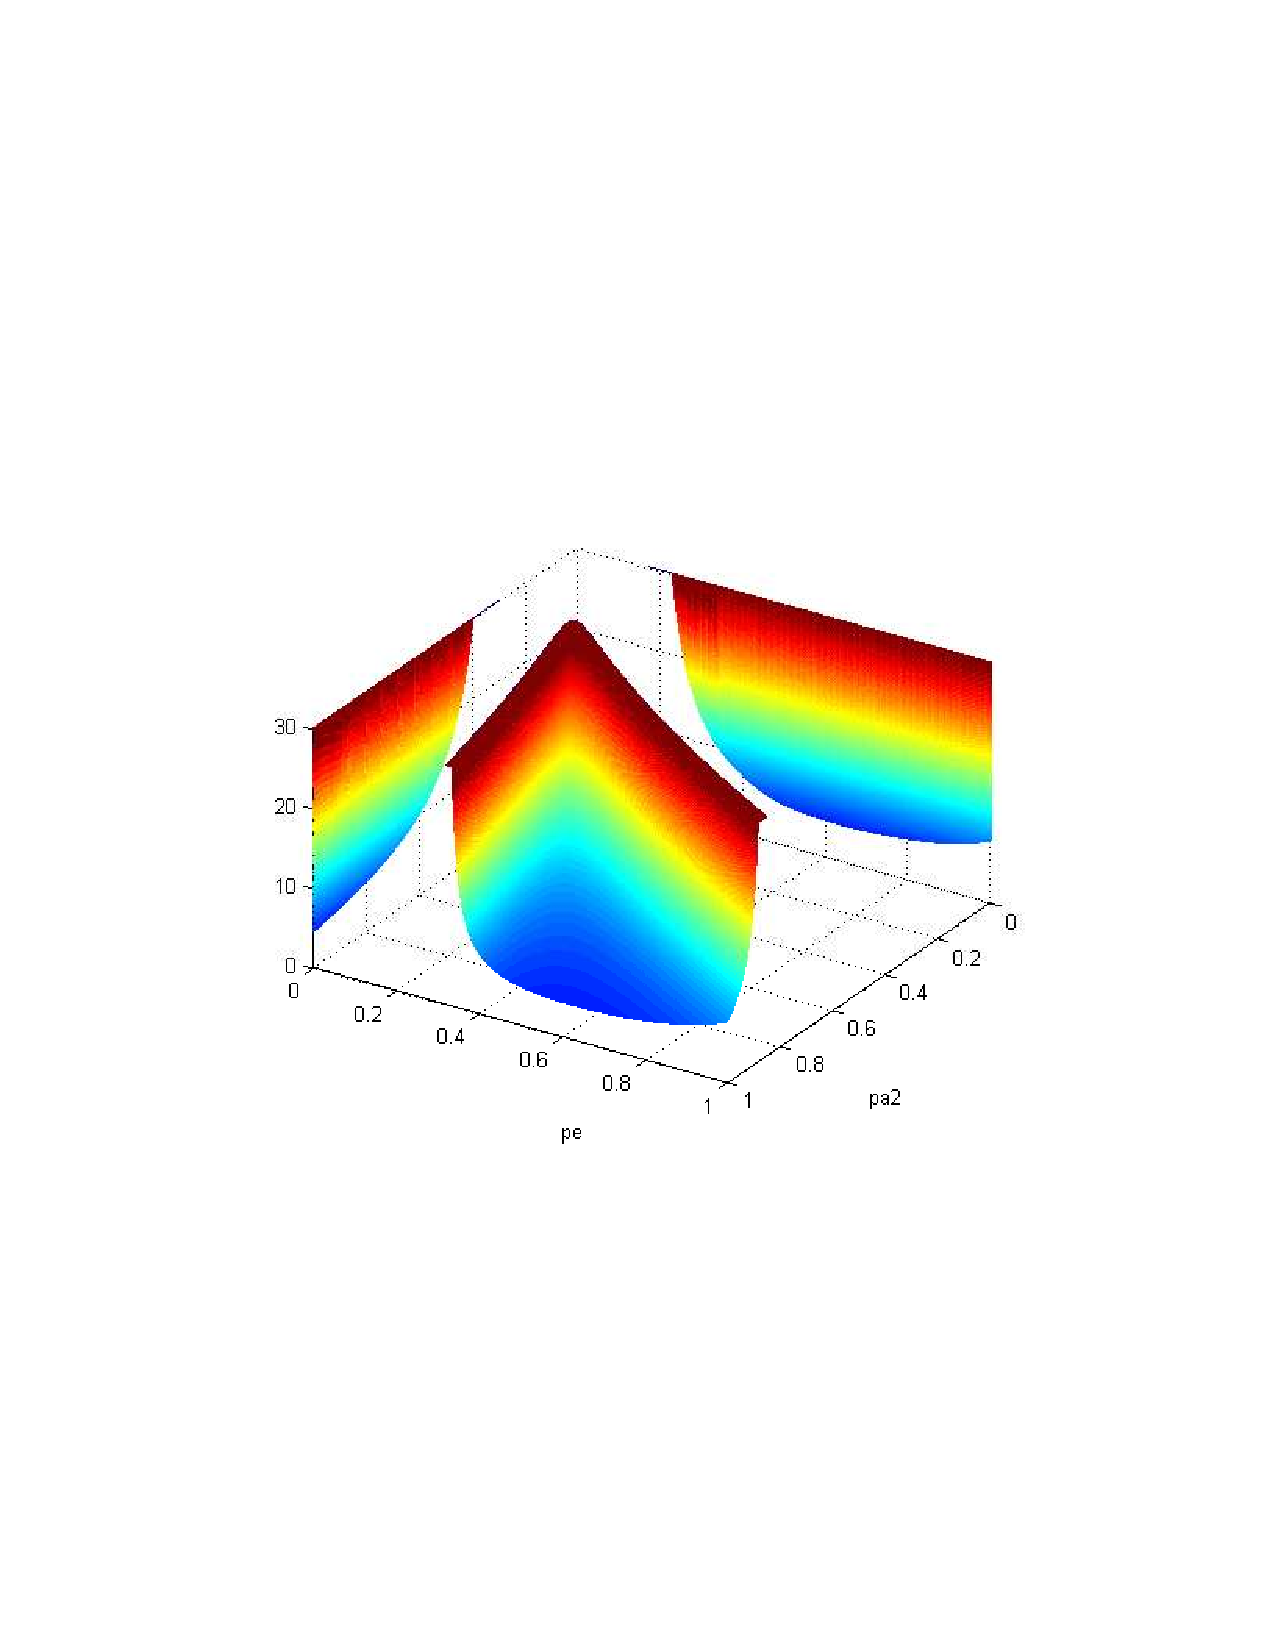
\includegraphics[width=2.5in]{pic/Gexpression.pdf}\\
%  \caption{the value of $G_e$ when $P_{a1} = 0.85$.}\label{fig:Gexpression}
%\end{figure}
%
%%
%%\begin{align}
%%Gexpression_{min} = \frac{(1-P_{a1})(3-P_{a1})}{(2-P_{a1})(1-M-P_{a1})-M}
%%\end{align}
%
%   So in this condition, the formula $E(T^{\mathcal{M}})-E(T^{\mathcal{C}}) \geq 0$ holds.
%Therefore when this condition is satisfied, conditional {\vwarm} strategy has better performance than the less {\vwarm} strategy.

%To prove the Theorem~\ref{lemma:warmnum2}, we need to compare $E(T^{\mathcal{M}})$ with $E(T^{\mathcal{C}})$.
%So we get the Formula~\ref{equ:tpc2}, and estimate if it is larger than $0$.
We estimate if it is greater than $0$.
First, we find that $P_{S_{\bar{c}, a}|S_{\bar{c},\bar{a}}^{\bar{w}}}^{\oplus} = P_{S_{\bar{c}, a}|S_{\bar{c},\bar{a}}}$.
Then by combing Equation~\ref{equ:pic} and ~\ref{equ:pim}, we get Equation~\ref{equ:ypwarm2} and \ref{equ:detail2}.
%For the calculation, $0 \leq P_{a1} \leq 1$, $0 \leq P_{a2} \leq 1$, $0 \leq P_{a2}^{'} \leq 1$, $0 \leq P_{a2}^{''} \leq 1$, $0 \leq P_{Lwarm} \leq 1$, $0 \leq P_{Mwarm} \leq 1$
% and $0 \leq P_{evict} \leq 1$.
%\begin{footnotesize}
\begin{equation}
\label{equ:ypwarm2}
\begin{split}
%\footnotesize
%\scriptsize
y(P_{w}^{\oplus}) = &B_{M}C_{M}P_{w}^{\oplus}+A_{M}C_{M}+GD_{M} \,
\end{split}\end{equation}
\begin{equation}
\label{equ:detail2}
\begin{split}
E(T^{\oplus}) - E(T) = &\frac{y(P_{w}^{\oplus})P_{w}^{\oplus}T_{w}}{E_{M}*F_{M}}
\end{split}\end{equation}
%\end{footnotesize}
where
\begin{equation*}
\begin{split}
&A_{M}= MG(1-P_{e|S_{c}})P_{S_{\bar{c}, a}|S_{\bar{c},\bar{a}}}+P_{e|S_{c}}(1-P_{a|S_{c}})\\
&B_{M}=MG(1-P_{e|S_{c}})(1-P_{S_{\bar{c}, a}|S_{\bar{c},\bar{a}}})\\
&C_{M}=P_{S_{\bar{c}, a}|S_{\bar{c},\bar{a}}}+P_{e|S_{c}}-P_{a|S_{c}}P_{e|S_{c}}\\
&D_{M}=P_{e|S_{c}}(P_{a|S_{c}}P_{S_{\bar{c}, a}|S_{\bar{c},\bar{a}}}+P_{a|S_{c}}P_{e|S_{c}}) \\
& \ \ \ \ \ \ \ \ -P_{e|S_{c}}((P_{a|S_{c}})^2P_{e|S_{c}}+P_{S_{\bar{c}, a}|S_{\bar{c},\bar{a}}})\\
&E_{M}=P_{e|S_{c}}+P_{w}^{\oplus}+P_{S_{\bar{c}, a}|S_{\bar{c},\bar{a}}}-P_{w}^{\oplus}P_{S_{\bar{c}, a}|S_{\bar{c},\bar{a}}} \\& \ \ \ \ \ \ \ \ -P_{e|S_{c}}(P_{w}^{\oplus}+P_{a|S_{c}}-P_{w}^{\oplus}P_{a|S_{c}})\\
&F_{M}=P_{S_{\bar{c}, a}|S_{\bar{c},\bar{a}}}+P_{e|S_{c}}(1-P_{a|S_{c}})
\end{split}\end{equation*}

Because $E_{M}$ and $F_{M}$ are greater than zero, to make $E(T^{\oplus}) - E(T) \geq 0$, $y(P_{w}^{\oplus})$ should be equal or greater than zero.
Therefore we can get $ B_{M}C_{M}P_{w}^{\oplus}+A_{M}C_{M}+GD_{M} \geq 0$.
If this inequality holds for all $P_{w}^{\oplus} \in [0,1]$, it should be satisfied that
\begin{equation}\label{equ:omega}
  (C_{M}(1-P_{e|S_{c}})P_{S_{\bar{c}, a}|S_{\bar{c},\bar{a}}}+D_{M})G+C_{M}P_{e|S_{c}}(1-P_{a|S_{c}}) \geq 0 \ .
\end{equation}
We denote $C_{M}(1-P_{e|S_{c}})P_{S_{\bar{c}, a}|S_{\bar{c},\bar{a}}}+D_{M}$ as $D_{F}$.
Therefore,
\begin{equation}
%\label{equ:detail2}
\begin{split}
D_{F} &=-(P_{e|S_{c}})^2(P_{a|S_{c}})^2+(P_{e|S_{c}})^2P_{a|S_{c}}  \\
&+(1-M(1-P_{e|S_{c}}))P_{e|S_{c}}P_{S_{\bar{c}, a}|S_{\bar{c},\bar{a}}}P_{a|S_{c}}\\
&+M(1-P_{e|S_{c}})(P_{e|S_{c}}+P_{S_{\bar{c}, a}|S_{\bar{c},\bar{a}}})P_{S_{\bar{c}, a}|S_{\bar{c},\bar{a}}}\\
&-P_{e|S_{c}}P_{S_{\bar{c}, a}|S_{\bar{c},\bar{a}}}
\end{split}\end{equation}

Regard $D_{F}$ as the function of $P_{a|S_{c}}$,
and we can find that it is an quadratic function.

When $P_{a|S_{c}} = 1$,
$$D_{F}(P_{a|S_{c}})=M(1-P_{e|S_{c}})(P_{S_{\bar{c}, a}|S_{\bar{c},\bar{a}}})^2 \geq 0 \ .$$

Let $D_{F}(P_{a|S_{c}}) = 0$,
 and denote the smaller root of the equation as $P_{a|S_{c},lroot}$.
  so when $P_{a|S_{c}} \geq P_{a|S_{c},lroot}$, $D_{F} \geq 0$.
   When $P_{a|S_{c}} < P_{a|S_{c},lroot}$, $D_{F} < 0$.
 Thus,
\begin{enumerate}
  \item
  When $P_{a|S_{c}} \geq P_{a|S_{c},lroot}$, $D_{F} \geq 0$.
  In this case, inequality \ref{equ:omega} holds. That is $E(T^{\oplus}) - E(T) \geq 0$.
  \item
  When $P_{a|S_{c}} < P_{a|S_{c},lroot}$, $D_{F} < 0$.
   In this case, to make the inequality \ref{equ:omega} holds,
   \begin{equation}\label{equ:ge}
     G \leq \frac{C_{M}P_{e|S_{c}}(P_{a|S_{c}}-1)}{D_{F}}
   \end{equation}
    for all $P_{e|S_{c}} \in [0,1]$ and $P_{S_{\bar{c}, a}|S_{\bar{c},\bar{a}}} \in [0,1]$.
\end{enumerate}

For the second case, denote
    $$F_G = \frac{C_{M}P_{e|S_{c}}(P_{a|S_{c}}-1)}{D_{F}}$$


\begin{enumerate}
\item
    First, we regard $F_G$ as the function of $P_{a|S_{c}}$ and calculate the derivative on $P_{a|S_{c}}$, and get:
    %\begin{equation*}
    \begin{flalign*}
    \frac{d(F_G)}{d(P_{a|S_{c}})} &= (P_{e|S_{c}})^{3}(1-P_{a|S_{c}})^2\\
    &\ \ \ \ \ \ +M(1-P_{e|S_{c}})P_{S_{\bar{c}, a}|S_{\bar{c},\bar{a}}}(P_{e|S_{c}}\\
    &\ \ \ \ \ \ +P_{S_{\bar{c}, a}|S_{\bar{c},\bar{a}}}-P_{e|S_{c}}P_{a|S_{c}})^{2}
    \end{flalign*}
    %\end{equation*}

Therefore,$\frac{d(F_G)}{d(P_{a|S_{c}})} \geq 0$, so that $F_G$ is a monotony increase function of $P_{a|S_{c}}$.
When $P_{a|S_{c}}$ fetches the minimum value, $F_G$ gets its minimum value.

\item
Second, we regard $F_G$ as the function of $P_{S_{\bar{c}, a}|S_{\bar{c},\bar{a}}}$ and calculate the derivative on $P_{S_{\bar{c}, a}|S_{\bar{c},\bar{a}}}$, and get:
\begin{equation*}
\begin{split}
&\frac{d(F_G)}{d(P_{S_{\bar{c}, a}|S_{\bar{c},\bar{a}}})} = \{M(1-P_{e|S_{c}})(1-P_{a|S_{c}})(P_{S_{\bar{c}, a}|S_{\bar{c},\bar{a}}}\\
&\ \ \  \ +P_{e|S_{c}}(1-P_{a|S_{c}}))^2-(P_{e|S_{c}})^2(1-P_{a|S_{c}})^2 \}P_{e|S_{c}}
\end{split}
\end{equation*}

Denote $P_{S_{\bar{c}, a}|S_{\bar{c},\bar{a}},rroot}$ as the greater root of equation $\frac{d(F_G)}{d(P_{S_{\bar{c}, a}|S_{\bar{c},\bar{a}}})}=0$.
\begin{equation*}
  P_{S_{\bar{c}, a}|S_{\bar{c},\bar{a}},rroot} = P_{e|S_{c}}\sqrt{\frac{1-P_{a|S_{c}}}{M(1-P_{e|S_{c}})}}-P_{e|S_{c}}(1-P_{a|S_{c}})
\end{equation*}
So, when $
0 \leq P_{S_{\bar{c}, a}|S_{\bar{c},\bar{a}}} \leq P_{S_{\bar{c}, a}|S_{\bar{c},\bar{a}},rroot}
$,
$$\frac{d(F_G)}{d(P_{S_{\bar{c}, a}|S_{\bar{c},\bar{a}}})} \leq 0 \ .$$

Therefore, when $P_{S_{\bar{c}, a}|S_{\bar{c},\bar{a}},rroot} \geq 1$, $F_G$ is a monotony decrease function of $P_{S_{\bar{c}, a}|S_{\bar{c},\bar{a}}}$.
When $P_{S_{\bar{c}, a}|S_{\bar{c},\bar{a}},rroot} < 1$, $F_G$ decreases at $[0,P_{S_{\bar{c}, a}|S_{\bar{c},\bar{a}},rroot}]$ and increases at $(P_{S_{\bar{c}, a}|S_{\bar{c},\bar{a}},rroot},1]$.

%$M(1+P_{evict})^{2} > 0$ and when $P_{a2} = 0$, so $\frac{d(Gexpression)}{d(P_{a2})} < 0$,
%$P_{a2r} > 0$.
%\begin{equation}
%\begin{split}
%P_{a2r}=\frac{P_{evict}\sqrt{\frac{(1+P_{evict})\bar{P}_{a1}}{M}}-P_{evict}\bar{P}_{a1}}{1+P_{evict}}
%\end{split}
%\end{equation}
%
%Therefore, if $P_{a2r} \geq 1$, then $\frac{d(Gexpression)}{d(P_{a2})} < 0$ and $Gexpression$ is a monotony decrease function of $P_{a2} \in [0,1]$.
%And if $P_{a2r} < 1$, then $Gexpression$ first decreases then increase as the function of $P_{a2} \in [0,1]$.
%
%Let $P_{a2r} = 1$, and we get:
%\begin{equation}
%\begin{split}
%\bar{P}_{a1}P_{evict}^3& + (\bar{P}_{a1}-M(1+\bar{P}_{a1})^2)P_{evict}^2\\
%& - 2M(\bar{P}_{a1}+1)P_{evict}-M = 0
%\end{split}
%\end{equation}
%It is a simple cubic equation on $P_{evict}$. We denote $P_{e\_r}$ as its greatest real root.
%If $P_{e\_r} < 1$,
%then, when $P_{evict} \geq P_{e\_r}$, $P_{a2r} \geq 1$. When $P_{evict} < P_{e\_r}$, $P_{a2r} < 1$.
%Otherwise, $P_{a2r} < 1$ holds.
%In general,if $P_{e\_r} < 1$, when $P_{evict} \geq P_{e\_r}$, $Gexpression$ is a monotony decrease function of $P_{a2} \in [0,1]$.
% When $P_{evict} < P_{e\_r}$, $Gexpression$ first decreases then increase as the function of $P_{a2} \in [0,1]$.
% And if not, $Gexpression$ first decreases then increase as the function of $P_{a2} \in [0,1]$.

\item
 Third, we regard $F_G$ as the function of $P_{e|S_{c}}$ and calculate the derivative on $P_{e|S_{c}}$, and get:
\begin{equation*}
\begin{split}
&\frac{d(F_G)}{d(P_{e|S_{c}})}=\\
&\ \ \ \ \ \ P_{S_{\bar{c}, a}|S_{\bar{c},\bar{a}}}(1-P_{a|S_{c}})(1-M+MP_{a|S_{c}})(P_{e|S_{c}})^2\\
&\ \ \ \ -2MP_{a|S_{c}}P_{S_{\bar{c}, a}|S_{\bar{c},\bar{a}}}(1-P_{S_{\bar{c}, a}|S_{\bar{c},\bar{a}}})P_{e|S_{c}}\\
&\ \ \ \ -M(P_{S_{\bar{c}, a}|S_{\bar{c},\bar{a}}})^3
\end{split}
\end{equation*}
When $P_{e|S_{c}} = 0$, $\frac{d(F_G)}{d(P_{e|S_{c}})} = -M(P_{S_{\bar{c}, a}|S_{\bar{c},\bar{a}}})^2 \leq 0 $.
Let $\frac{d(F_G)}{d(P_{e|S_{c}})} = 0$, we can get the right root of this equation:
\begin{equation}
\begin{split}
P_{e|S_{c},rroot} &= \frac{MP_{a|S_{c}}(1-P_{S_{\bar{c}, a}|S_{\bar{c},\bar{a}}})+\sqrt{\Delta}}{(1-P_{a|S_{c}})(1-M+MP_{a|S_{c}})}
\end{split}
\end{equation}
where
\begin{align}
\Delta = &M^{2}(P_{a|S_{c}})^{2}(1-P_{S_{\bar{c}, a}|S_{\bar{c},\bar{a}}})^2 \nonumber \\
&+ M(P_{S_{\bar{c}, a}|S_{\bar{c},\bar{a}}})^{2}(1-P_{a|S_{c}})(1-M+MP_{a|S_{c}})\  .\nonumber
\end{align}
So when
$
0 \leq P_{e|S_{c}} \leq P_{e|S_{c},rroot}
$,
$$\frac{d(F_G)}{d(P_{e|S_{c}})} \leq 0\ .$$

Therefore, when $P_{e|S_{c},rroot} \geq 1$, $F_G$ is a monotony decrease function of $P_{e|S_{c}}$.
When $P_{e|S_{c},rroot} < 1$, $F_G$ decreases at $[0,P_{e|S_{c},rroot}]$ and increases at $(P_{e|S_{c},rroot},1]$.

%If $P_{a2}=\sqrt{\frac{\bar{P}_{a1}}{M}}-\bar{P}_{a1}$, $\frac{d(Gexpression)}{d(P_{evict})} < 0$. Function $Gexpression$ is a monotony decrease function on $P_{evict}$.
%Otherwise, $\frac{d(Gexpression)}{d(P_{evict})}$ is a simple cubic equation on $P_{evict}$.
%The symmetry axis of the function $\frac{d(Gexpression)}{d(P_{evict})}$ is:
%\begin{equation}
%\begin{split}
%P_{e\_axis}=\frac{MP_{a2}(\bar{P}_{a1}+P_{a2})}{\bar{P}_{a1}-M(\bar{P}_{a1}+P_{a2})^2}
%\end{split}
%\end{equation}
%(1) If $P_{a2}< \sqrt{\frac{\bar{P}_{a1}}{M}}-\bar{P}_{a1}$,
% then $P_{e\_axis} > 0$.
%
% When $P_{evict} = 0$, $\frac{d(Gexpression)}{d(P_{evict})} = -MP_{a2}^3 < 0$.
% When $P_{evict} = 1$,
% $$
% \frac{d(Gexpression)}{d(P_{evict})} = P_{a2}(\bar{P}_{a1}-M(\bar{P}_{a1}+2P_{a2})^2)
% $$
%So when $P_{a2}< \frac{1}{2}(\sqrt{\frac{\bar{P}_{a1}}{M}}-\bar{P}_{a1})$, $\frac{d(Gexpression)}{d(P_{evict})} > 0$.
% In this case, $Gexpression$ first decreases then increase as the function of $P_{evict} \in [0,1]$.
%when $P_{a2}\geq \frac{1}{2}(\sqrt{\frac{\bar{P}_{a1}}{M}}-\bar{P}_{a1})$, $\frac{d(Gexpression)}{d(P_{evict})} < 0$.
% In this case, $Gexpression$ is a  a monotony decrease function of $P_{evict} \in [0,1]$.
%(2) If $P_{a2}> \sqrt{\frac{\bar{P}_{a1}}{M}}-\bar{P}_{a1}$,
%then $P_{e\_axis} < 0$.
% When $P_{evict} = 0$, $\frac{d(Gexpression)}{d(P_{evict})} = -MP_{a2}^3 < 0$.
%So in this case, $Gexpression$ is a  a monotony decrease function of $P_{evict} \in [0,1]$.

%In general, when $P_{a2}< \frac{1}{2}(\sqrt{\frac{\bar{P}_{a1}}{M}}-\bar{P}_{a1})$, $Gexpression$ first decreases then increase as the function of $P_{evict} \in [0,1]$; when $P_{a2}\geq \frac{1}{2}(\sqrt{\frac{\bar{P}_{a1}}{M}}-\bar{P}_{a1})$, $Gexpression$ is a  a monotony decrease function of $P_{evict} \in [0,1]$.
%
%In a conclusion, if $GDenominator > 0$,
%$Gexpression$ is a monotony increase function of $P_{a1}$;
% when $P_{evict} < \min(P_{e\_r},1)$, $Gexpression$ first decreases then increase as the function of $P_{a2} \in [0,1]$;
% if $P_{e\_r} < 1$, when $P_{evict} \geq P_{e\_r}$, $Gexpression$ is a monotony decrease function of $P_{a2} \in [0,1]$;
%when $P_{a2}< \frac{1}{2}(\sqrt{\frac{\bar{P}_{a1}}{M}}-\bar{P}_{a1})$, $Gexpression$ first decreases then increase as the function of $P_{evict} \in [0,1]$; when $P_{a2}\geq \frac{1}{2}(\sqrt{\frac{\bar{P}_{a1}}{M}}-\bar{P}_{a1})$, $Gexpression$ is a  a monotony decrease function of $P_{evict} \in [0,1]$.
%
%Therefore, the minimum value of $Gexpression$ is get when $P_{a1}$ achieves the minimum value, $P_{a2}$ and $P_{evict}$ achieve the maximum value.
\end{enumerate}

Therefore, the minimum value of $F_G$ gets when
\begin{equation}
\left\{
\begin{split}
&P_{e|S_{c}} = \frac{MP_{a|S_{c}}(1-P_{S_{\bar{c}, a}|S_{\bar{c},\bar{a}}})+\sqrt{\Delta}}{(1-P_{a|S_{c}})(1-M+MP_{a|S_{c}})} \\
&P_{S_{\bar{c}, a}|S_{\bar{c},\bar{a}}} = P_{e|S_{c}}\sqrt{\frac{1-P_{a|S_{c}}}{M(1-P_{e|S_{c}})}}-P_{e|S_{c}}(1-P_{a|S_{c}}) \\
& if\  P_{e|S_{c}} >1, P_{e|S_{c}} = 1 \\
& if\  P_{S_{\bar{c}, a}|S_{\bar{c},\bar{a}}} >1, P_{S_{\bar{c}, a}|S_{\bar{c},\bar{a}}} = 1
\end{split}
\right.
\end{equation}

From the above, we can make the following conclusions:
\begin{enumerate}
  \item
  When $D_F \geq 0$, $E(T^{\oplus}) - E(T) \geq 0$.
  \item
  When $D_F < 0$, $E(T^{\oplus}) - E(T) \geq 0$ if $G$ is smaller than the minimum value of $F_G$.
\end{enumerate}

That is:
$\forall D_F$, when  $D_F < 0$, $G$ is less than the minimum value of $F_G$.
At this point conditional {\vwarm} strategy has better performance than the less {\vwarm} strategy.




%The symmetry axis of $y(P_{warm})$ is $P_{warm} = P_{a}$, where $P_{a}$ is denoted in Equation~\ref{equ:pa}.
%%\begin{footnotesize}
%\begin{equation}
%\label{equ:pa}
%\begin{split}
%P_{a} = &\frac{1}{2(P_{evict}+P_{delay})}\{k*P_{evict}P_{delay}\\
%& + P_{evict}^{2}P_{delay} \\
%&+ P_{evict}P_{delay}^{2} - P_{evict}^{2} \\
%& - P_{evict}P_{delay}\} \ .
%\end{split}
%\end{equation}
%%\end{footnotesize}
%Equation~\ref{equ:pal0} holds when $0.8 \leq P_{delay} \leq 1$, $0 \leq P_{evict} \leq 1$,  which means $P_{a}  \geq 0$.
%%\begin{footnotesize}
%  \begin{equation}
%  \label{equ:pal0}
%  \begin{split}
%     k  > 1 > & \frac{P_{evict}^{2} + P_{evict}P_{delay} - P_{evict}P_{delay}^{2} - P_{evict}^{2}P_{delay}}{P_{evict}P_{delay}} \\
%     &=1+ \frac{P_{evict}}{P_{delay}} - P_{delay} - P_{evict} \ .
%  \end{split}
%  \end{equation}
% % \end{footnotesize}
%  %We make $k_{1} = \frac{P_{evict}^{2} + P_{evict}P_{delay} - P_{evict}P_{delay}^{2} - P_{evict}^{2}P_{delay}}{P_{evict}P_{delay}}$.
%  %After simplified, $k_{1} = \frac{P_{evict}}{P_{delay}} - P_{delay} + 1 - P_{evict}$.
%  %$k_{1}$ is a decreasing function of $P_{delay}$, the maximum of $k_{1}$ is $0.25P_{evict}+0.2$ when $P_{delay} = 0.8$. The maximum value is less than 1, but $k$ must be larger than $1$. So this condition is false.
% %means $k<1$ which conflicts with the precondition $k>1$.
%
%
%
%\begin{enumerate}
%
%
%  \item If $P_{a} > 1$ (i.e., Equation~\ref{equ:pal1} holds), the minimum value of $y(P_{warm})$ is $y(1)$.
%  When $k \epsilon (k_{1}, k_{0}]$, $y(P_{warm}) \geq 0$ holds.
%  %\begin{footnotesize}
%    \begin{equation}
%    \label{equ:pal1}
%     k_{1} = \frac{(P_{evict}+P_{delay})(2+P_{evict}-P_{delay}P_{evict})}{P_{evict}P_{delay}} \ .
%  \end{equation}
%  %\end{footnotesize}
%  %In this condition,.
% % \begin{equation}
%  %  \scriptsize
%  %  y(1) = (P_{delay} - 1)P_{evict}P_{delay}k + (1 + P_{evict}- P_{evict}P_{delay})(P_{evict}+P_{delay}) \ .
% % \end{equation}
%  %make $y(1) \geq 0$, so all $y(P_{warm}) \geq 0$ when $0 \leq P_{warm} \leq 1$ . So:
%  %\begin{footnotesize}
%  \begin{equation}
%   k_{0} = \frac{(1 + P_{evict}- P_{evict}P_{delay})(P_{evict}+P_{delay})}{(1 - P_{delay})P_{evict}P_{delay}}\ .
%  \end{equation}
%  %\end{footnotesize}
%  %We mark $k_{2} = \frac{(P_{evict}+P_{delay})(2+P_{evict}-P_{delay}P_{evict})}{P_{evict}P_{delay}}$ and \par $k_{0} = \frac{(1 + P_{evict}- P_{evict}P_{delay})(P_{evict}+P_{delay})}{(1 - P_{delay})P_{evict}P_{delay}}$ ,\par so when
%  %$k_{2} < k \leq k_{0},$
% % $$y(P_{warm}) \geq 0$$.\par
%
% % \ \par
%
%  \item If $0 \leq P_{a} \leq 1,$ (i.e., $1 < k \leq k_{1}$), the minimum value of $y(P_{warm})$ is $y(P_{a})$.
%  %\begin{scriptsize}
%  \begin{equation}\begin{split}
%    %\scriptsize
%    &y(P_{a}) = \frac{1}{4(P_{evict}+P_{delay})}\{-P_{evict}^{2}P_{delay}^{2}k^{2}\\
%    &+ 2P_{evict}^{2}P_{delay}(2P_{delay}+P_{evict}-P_{evict}P_{delay})k\\
%    &+ 2P_{evict}P_{delay}^{2}(2P_{delay}+P_{evict}-P_{evict}P_{delay})k\\
%    & - P_{evict}^{2}(P_{evict}+P_{delay})^{2}(1-P_{delay})^{2}\}.
%  \end{split}\end{equation}
%%\end{scriptsize}
% $y(P_{a})$ is a function of $k$ (denoted as $f(k)$). As $-P_{evict}^{2}P_{delay}^{2} < 0$, the minimum of $f(k)$ is either $f(1)$ or $f(k_{1})$, for $1 < k \leq k_{1}$. When $P_{delay} \in [0.8,1]$, $f(1)$ and  $f(k_{2})$ is larger than $0$, which means $y(P_{a}) > 0$
%
%  % So if $f(1)>0 and f(k_{2})>0$, $f(k)>0 in k \in (1,k_{2}]$.
%  %\begin{scriptsize}
%  \begin{equation}
%  \label{equ:f1}
%  \begin{split}
%    %\scriptsize
%    f(1) =& \frac{1}{4(P_{evict}+P_{delay})}\{-(1-P_{delay})^{2}P_{evict}^{4}\\ & + 2P_{evict}^{3}P_{delay}^{2} + 4P_{evict}P_{delay}^{3} \\ &+ P_{evict}^{2}P_{delay}^{2}(4-P_{delay}^{2} - 2P_{evict}P_{delay})\}.
%  \end{split}\end{equation}%\end{scriptsize}
% % So, $f(1) > 0$ is true when $P_{delay} \in [0.8,1]$.
%
%  %\begin{footnotesize}
%  \begin{equation}
%  \label{equ:fk1}
%    \raggedleft
%  \begin{split}
%    f(k_{1}) = &(P_{evict}+P_{delay})\{2P_{delay}- 1\\ & + P_{evict}P_{delay}(1 - P_{delay})\}.
%  \end{split}\end{equation}
%  %\end{footnotesize}
%  %So, $f(k_{2}) > 0$ is true when $P_{delay} \in [0.8,1]$.\par
%
% % \ \par
%
%  %Therefore, when $1< k \leq k_{2}$, $y(P_{a}) > 0$.
%
%  %So, $y(P_{warm}) > 0$.
%
%\end{enumerate}
%%So, we can get that when $1< k \leq k_{0}$, $y(P_{warm}) \geq 0$.
%From the above analysis, we find that when $1< k \leq k_{0}$, $E(T^{p}) \geq E(T^{c})$.
%%I.e. when $1< k \leq k_{0}$, $T^{p} \geq T^{C}$

\section{$P_{a}$ for Different AES Key Lengthes and Implementations}
\label{appendixb}
We assume the size of a cache line is $C$ Byte. $P_{a}$ represents that the probability that some of the $N$ cache line size of lookup tables not in the cache are accessed. So when the AES implementation uses 4.25KB lookup tables, the $P_{a}$ for AES-128, AES-192 and AES-256 are as follows respectively:
\begin{align}
%\begin{flalign}
%\begin{split}
    P_{a}^{128} = &1-   \nonumber \\
    \frac{1}{\binom{4352/C}{N}}&\sum_{x_4=x_{4b}}^{x_{4e}}{\sum_{x_0=x_{0b}}^{x_{0e}}{\sum_{x_1=x_{1b}}^{x_{1e}}{ \sum_{x_2=x_{2b}}^{x_{2e}}{f(x_4)\prod_{i=0}^{3}{g(x_i,36)}}}}}, \nonumber
%\end{split}
%\end{flalign}
\end{align}
%for AES-192 is
\begin{align}
    %\scriptsize
    P_{a}^{192} = &1-  \nonumber \\
    \frac{1}{\binom{4352/C}{N}}&\sum_{x_4=x_{4b}}^{x_{4e}}{\sum_{x_0=x_{0b}}^{x_{0e}}{\sum_{x_1=x_{1b}}^{x_{1e}}{ \sum_{x_2=x_{2b}}^{x_{2e}}{f(x_4)\prod_{i=0}^{3}{g(x_i,44)}}}}}, \nonumber
\end{align}
%for AES-256 is
\begin{align}
    %\scriptsize
    P_{a}^{256} = &1-  \nonumber \\
    \frac{1}{\binom{4352/C}{N}}&\sum_{x_4=x_{4b}}^{x_{4e}}{\sum_{x_0=x_{0b}}^{x_{0e}}{\sum_{x_1=x_{1b}}^{x_{1e}}{ \sum_{x_2=x_{2b}}^{x_{2e}}{f(x_4)\prod_{i=0}^{3}{g(x_i,52)}}}}}, \nonumber
\end{align}

%\begin{equation}
%    %\scriptsize
%    P_{delay}^{128} = 1- \frac{1}{\binom{68}{N}}\sum_{x_4=\max(0,N-64)}^{\min(4,N)}{\sum_{x_0=\max(0,N-x_4-48)}^{\min(16,N-x_4)}{\sum_{x_1=\max(0,N-x_4-x_0-32)}^{\min(16,N-x_4-x_0)}{ \sum_{x_2=\max(0,N-x_4-x_0-x_1-16)}^{min(16,N-x_4-x_0-x_1)}{\binom{4}{x_4}(1-\frac{x_4}{4})^{16}\prod_{i=0}^{3}{\binom{16}{x_i}(1-\frac{x_i}{16})^{36}}}}}},
%\end{equation}
%%for AES-192 is
%\begin{equation}
%    %\scriptsize
%    P_{delay}^{192} = 1- \frac{1}{\binom{68}{N}}\sum_{x_4=\max(0,N-64)}^{\min(4,N)}{\sum_{x_0=\max(0,N-x_4-48)}^{\min(16,N-x_4)}{\sum_{x_1=\max(0,N-x_4-x_0-32)}^{\min(16,N-x_4-x_0)}{ \sum_{x_2=\max(0,N-x_4-x_0-x_1-16)}^{min(16,N-x_4-x_0-x_1)}{\binom{4}{x_4}(1-\frac{x_4}{4})^{16}\prod_{i=0}^{3}{\binom{16}{x_i}(1-\frac{x_i}{16})^{44}}}}}},
%\end{equation}
%%for AES-256 is
%\begin{equation}
%    %\scriptsize
%    P_{delay}^{256} = 1- \frac{1}{\binom{68}{N}}\sum_{x_4=\max(0,N-64)}^{\min(4,N)}{\sum_{x_0=\max(0,N-x_4-48)}^{\min(16,N-x_4)}{\sum_{x_1=\max(0,N-x_4-x_0-32)}^{\min(16,N-x_4-x_0)}{ \sum_{x_2=\max(0,N-x_4-x_0-x_1-16)}^{min(16,N-x_4-x_0-x_1)}{\binom{4}{x_4}(1-\frac{x_4}{4})^{16}\prod_{i=0}^{3}{\binom{16}{x_0}(1-\frac{x_i}{16})^{52}}}}}}.
%\end{equation}

where
  \begin{eqnarray*}
  % \nonumber to remove numbering (before each equation)
    &&f(x) = \binom{256/C}{x}(1-\frac{xC}{256})^{16} \\
    &&g(x,y) = \binom{1024/C}{x}(1-\frac{xC}{1024})^{y} \\
    &&x_0+x_1+x_2+x_3+x_4 = N \\
    &&x_{4b} = \max(0,N-4096/C) \\
    &&x_{4e} = \min(256/C,N) \\
    &&x_{0b} = \max(0,N-x_4-3072/C) \\
    &&x_{0e} = \min(1024/C,N-x_4) \\
    &&x_{1b} = \max(0,N-x_4-x_0-2048/C) \\
    &&x_{1e} = \min(1024/C,N-x_4-x_0) \\
    &&x_{2b} = \max(0,N-x_4-x_0-x_1-1024/C) \\
    &&x_{2e} = \min(1024/C,N-x_4-x_0-x_1)
  \end{eqnarray*}

When the AES implementation uses 5KB lookup tables, the $P_{a}$ for AES-128, AES-192 and AES-256 are as follows respectively:
\begin{align}
    P_{a}^{128} = &1-   \nonumber \\
    \frac{1}{\binom{5120/C}{N}}&\sum_{x_4=x_{4b}}^{x_{4e}}{\sum_{x_0=x_{0b}}^{x_{0e}}{\sum_{x_1=x_{1b}}^{x_{1e}}{ \sum_{x_2=x_{2b}}^{x_{2e}}{f(x_4,16)\prod_{i=0}^{3}{f(x_i,36)}}}}}, \nonumber
\end{align}
%for AES-192 is
\begin{align}
    %\scriptsize
    P_{a}^{192} = &1-  \nonumber \\
    \frac{1}{\binom{5120/C}{N}}&\sum_{x_4=x_{4b}}^{x_{4e}}{\sum_{x_0=x_{0b}}^{x_{0e}}{\sum_{x_1=x_{1b}}^{x_{1e}}{ \sum_{x_2=x_{2b}}^{x_{2e}}{f(x_4,16)\prod_{i=0}^{3}{f(x_i,44)}}}}}, \nonumber
\end{align}
%for AES-256 is
\begin{align}
    %\scriptsize
    P_{a}^{256} = &1-  \nonumber \\
    \frac{1}{\binom{5120/C}{N}}&\sum_{x_4=x_{4b}}^{x_{4e}}{\sum_{x_0=x_{0b}}^{x_{0e}}{\sum_{x_1=x_{1b}}^{x_{1e}}{ \sum_{x_2=x_{2b}}^{x_{2e}}{f(x_4,16)\prod_{i=0}^{3}{f(x_i,52)}}}}}, \nonumber
\end{align}
where
  \begin{eqnarray*}
  % \nonumber to remove numbering (before each equation)
    &&f(x,y) = \binom{1024/C}{x}(1-\frac{xC}{1024})^{y} \\
    &&x_0+x_1+x_2+x_3+x_4 = N \\
    &&x_{4b} = \max(0,N-4096/C) \\
    &&x_{4e} = \min(1024/C,N) \\
    &&x_{0b} = \max(0,N-x_4-3072/C) \\
    &&x_{0e} = \min(1024/C,N-x_4) \\
    &&x_{1b} = \max(0,N-x_4-x_0-2048/C) \\
    &&x_{1e} = \min(1024/C,N-x_4-x_0) \\
    &&x_{2b} = \max(0,N-x_4-x_0-x_1-1024/C) \\
    &&x_{2e} = \min(1024/C,N-x_4-x_0-x_1)
  \end{eqnarray*}

%\begin{equation}
%    %\scriptsize
%    P_{delay}^{128} = 1- \frac{1}{\binom{80}{N}}\sum_{x_4=\max(0,N-64)}^{\min(16,N)}{\sum_{x_0=\max(0,N-x_4-48)}^{\min(16,N-x_4)}{\sum_{x_1=\max(0,N-x_4-x_0-32)}^{\min(16,N-x_4-x_0)}{ \sum_{x2=\max(0,N-x_4-x_0-x_1-16)}^{min(16,N-x_4-x_0-x_1)}{\binom{16}{x_4}\binom{16}{x_0}\binom{16}{x_1}\binom{16}{x_2}\binom{16}{x_3}} (1-\frac{x_4}{16})^{16}\prod_{i=0}^{3}{(1-\frac{x_i}{16})^{36}}}}},
%\end{equation}
%%for AES-192 is
%\begin{equation}
%    %\scriptsize
%    P_{delay}^{192} = 1- \frac{1}{\binom{80}{N}}\sum_{x_4=\max(0,N-64)}^{\min(16,N)}{\sum_{x_0=\max(0,N-x_4-48)}^{\min(16,N-x_4)}{\sum_{x_1=\max(0,N-x_4-x_0-32)}^{\min(16,N-x_4-x_0)}{ \sum_{x_2=\max(0,N-x_4-x_0-x_1-16)}^{min(16,N-x_4-x_0-x_1)}{\binom{16}{x_4}\binom{16}{x_0}\binom{16}{x_1}\binom{16}{x_2}\binom{16}{x_3}} (1-\frac{x_4}{16})^{16}\prod_{i=0}^{3}{(1-\frac{x_i}{16})^{44}}}}},
%\end{equation}
%%for AES-256 is
%\begin{equation}
%    %\scriptsize
%    P_{delay}^{256} = 1- \frac{1}{\binom{80}{N}}\sum_{x_4=\max(0,N-64)}^{\min(16,N)}{\sum_{x_0=\max(0,N-x_4-48)}^{\min(16,N-x_4)}{\sum_{x_1=\max(0,N-x_4-x_0-32)}^{\min(16,N-x_4-x_0)}{ \sum_{x_2=\max(0,N-x_4-x_0-x_1-16)}^{min(16,N-x_4-x_0-x_1)}{\binom{16}{x_4}\binom{16}{x_0}\binom{16}{x_1}\binom{16}{x_2}\binom{16}{x_3}} (1-\frac{x_4}{16})^{16}\prod_{i=0}^{3}{(1-\frac{x_i}{16})^{52}}}}}.
%\end{equation}
%where
%\begin{equation*}
%  x_0+x_1+x_2+x_3+x_4=N.
%\end{equation*}

When the AES implementation uses 4KB lookup tables, the $P_{a}$ for AES-128, AES-192 and AES-256 are as follows respectively:
\begin{align}
    P_{a}^{128} = &1-   \nonumber \\
    \frac{1}{\binom{4096/C}{N}}&\sum_{x_0=x_{0b}}^{x_{0e}}{\sum_{x_1=x_{1b}}^{x_{1e}}{\sum_{x_2=x_{2b}}^{x_{2e}}{\prod_{i=0}^{3}{f(x_i,40)}}}}, \nonumber
\end{align}
%for AES-192 is
\begin{align}
    %\scriptsize
    P_{a}^{192} = &1-  \nonumber \\
    \frac{1}{\binom{4096/C}{N}}&\sum_{x_0=x_{0b}}^{x_{0e}}{\sum_{x_1=x_{1b}}^{x_{1e}}{\sum_{x_2=x_{2b}}^{x_{2e}}{\prod_{i=0}^{3}{f(x_i,48)}}}}, \nonumber
\end{align}
%for AES-256 is
\begin{align}
    %\scriptsize
    P_{a}^{256} = &1-  \nonumber \\
    \frac{1}{\binom{4096/C}{N}}&\sum_{x_0=x_{0b}}^{x_{0e}}{\sum_{x_1=x_{1b}}^{x_{1e}}{\sum_{x_2=x_{2b}}^{x_{2e}}{\prod_{i=0}^{3}{f(x_i,56)}}}}, \nonumber
\end{align}
where
  \begin{eqnarray*}
  % \nonumber to remove numbering (before each equation)
    &&f(x,y) = \binom{1024/C}{x}(1-\frac{xC}{1024})^{y} \\
    &&x_0+x_1+x_2+x_3 = N \\
    &&x_{0b} = \max(0,N-3072/C) \\
    &&x_{0e} = \min(1024/C,N) \\
    &&x_{1b} = \max(0,N-x_0-2048/C) \\
    &&x_{1e} = \min(1024/C,N-x_0) \\
    &&x_{2b} = \max(0,N-x_0-x_1-1024/C) \\
    &&x_{2e} = \min(1024/C,N-x_0-x_1)
  \end{eqnarray*}

%\begin{equation}
%    %\scriptsize
%    P_{delay}^{128} = 1- \frac{1}{\binom{64}{N}}\sum_{x_0=\max(0,N-48)}^{\min(16,N)}{\sum_{x_1=\max(0,N-x_0-32)}^{\min(16,N-x_0)}{ \sum_{x_2=\max(0,N-x_0-x_1-16)}^{min(16,N-x_0-x_1)}{\binom{16}{x_0}\binom{16}{x_1}\binom{16}{x_2}\binom{16}{x_3}} \prod_{i=0}^{3}{(1-\frac{x_i}{16})^{40}}}},
%\end{equation}
%%for AES-192 is
%\begin{equation}
%    %\scriptsize
%    P_{delay}^{192} = 1- \frac{1}{\binom{64}{N}}\sum_{x_0=\max(0,N-48)}^{\min(16,N)}{\sum_{x_1=\max(0,N-x_0-32)}^{\min(16,N-x_0)}{ \sum_{x_2=\max(0,N-x_0-x_1-16)}^{min(16,N-x_0-x_1)}{\binom{16}{x_0}\binom{16}{x_1}\binom{16}{x_2}\binom{16}{x_3}} \prod_{i=0}^{3}{(1-\frac{x_i}{16})^{48}}}},
%\end{equation}
%%for AES-256 is
%\begin{equation}
%    %\scriptsize
%    P_{delay}^{256} = 1- \frac{1}{\binom{64}{N}}\sum_{x_0=\max(0,N-48)}^{\min(16,N)}{\sum_{x_1=\max(0,N-x_0-32)}^{\min(16,N-x_0)}{ \sum_{x_2=\max(0,N-x_0-x_1-16)}^{min(16,N-x_0-x_1)}{\binom{16}{x_0}\binom{16}{x_1}\binom{16}{x_2}\binom{16}{x_3}} \prod_{i=0}^{3}{(1-\frac{x_i}{16})^{56}}}}.
%\end{equation}
%where
%\begin{equation*}
%  x_0+x_1+x_2+x_3=N.
%\end{equation*}

When the AES implementation uses 2KB lookup table, the $P_{a}$ for AES-128, AES-192 and AES-256 are as follows respectively:
\begin{equation*}
    %\scriptsize
    P_{a}^{128} = 1- (1-\frac{NC}{2048})^{16*10},
\end{equation*}
%for AES-192 is
\begin{equation*}
    %\scriptsize
    P_{a}^{192} = 1- (1-\frac{NC}{2048})^{16*12},
\end{equation*}
%for AES-256 is
\begin{equation*}
    %\scriptsize
    P_{a}^{256} = 1- (1-\frac{NC}{2048})^{16*14}.
\end{equation*}
